

\chapter{Preliminaries}

In this chapter we intend to provide technical and teoretical background for terms, which will be used in the thesis. We describe used dataset for evaluations, some technical terms later used and we provide a quick overview of Deep Neural Networks.

\begin{figure}
	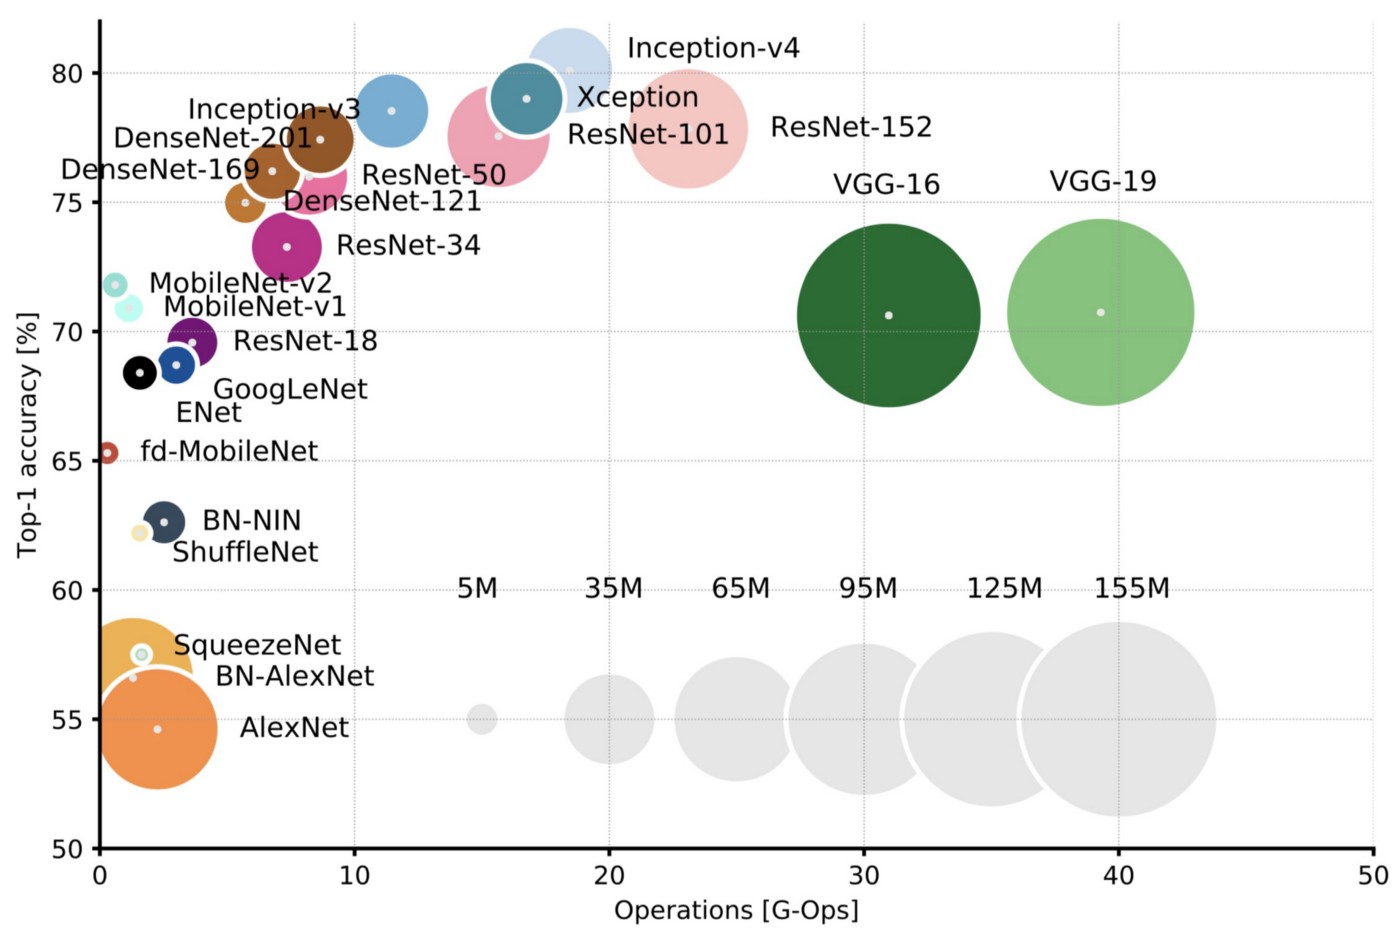
\includegraphics[width=0.8\linewidth]{img/network-comparison.jpeg}
	\caption{Top-1 one-crop accuracy versus amount of operations required for a single forward pass. The size of the blobs is proportional to the number of network parameters. Source: \cite{canziani2016analysis}}
	\label{fig:camera-setup}
\end{figure}


\section{Distance Measures}

\subsection{Cosine Distance}
\begin{equation}
similarity = \cos ({\bf t},{\bf e})= {{\bf t} {\bf e} \over \|{\bf t}\| \|{\bf e}\|} = \frac{ \sum_{i=1}^{n}{{\bf t}_i{\bf e}_i} }{ \sqrt{\sum_{i=1}^{n}{{\bf t}_i^2}} \sqrt{\sum_{i=1}^{n}{{\bf e}_i^2}} }
\end{equation}
\begin{equation}
    distance = 1 - similarity
\end{equation}

\subsection{Euclidean Distance}
\begin{equation}
d(p, q) = \sqrt{\sum_{i=1}^n (p_i - q_i)^2}    
\end{equation}

\section{Dataset}

We use Vimeo Creative Commons Collections (V3C1)\footnote{\href{https://www-nlpir.nist.gov/projects/tv2019/data.html}{TRECVID 2019 Video Data}} as our dataset for evaluation. This dataset is composed of 7475 Vimeo videos. For our purposes we use only first 750 videos out of this dataset. From these, we used an extraction tool from VIRET \cite{lokovc2019framework}. Via extraction we obtained \todo{fix}111\ 400 images from 750 videos with resolution 320x180.

The variety of captured scenes and occasions in the videos is large. In many of them we can see different landscapes. From seas to mountain view, from desert to snow. One \todo{fix}tenth of the videos contain people in it. These people also cover wide range of activities, from Hindi wedding, to skateboarding in a park or a news broadcast.

\subsection{Collages}



\section{Intersection over Union}

In the following chapter we use Intersection over Union (IoU) as a characteristic of overlaping. Intersection over Union (also known as Jaccard index\footnote{\href{https://en.wikipedia.org/wiki/Jaccard_index}{https://en.wikipedia.org/wiki/Jaccard\_index}}) measures similarity between two sets. In our case, we use is as a metric to express how much two regions (i.e. two rectangles) overlap. A visual hint over the meaning can be seen in Figure \ref{fig:intersection_over_union}
\todo[inline]{Vzorec}

\section{Deep Neural Networks}

In the recent years we witnessed many records-breaking new machine learning models. Many of those were possible thanks to advancement of Deep Neural Networks (DNN). Nowadays, these model replaced more traditional Machine Learning approaches in many tasks.

Deep Neural Network is a machine learning model, which goal is to approximate a given function \(f\). Set of parameters is often refered as \(\theta\). One of the common tasks performed by these networks is classification, where the goal of the network is to predict to which category sample \(X\) belongs. Even though, we will not perform classification task in this thesis, we will use some of the available classification networks.

When we talk about neural networks, we usually refer to feedforward network. These networks consist of set of the layers, where information during the evaluation is passed only in one direction. This can be imagined as an applying a function on the results from the previous layer. In example, let's create a small neural network. Denote first layer as \(f_1\) and second layer as \(f_2\). The output of the network will be \(f_2\left(f_1\left(\right)\right)\).

Stacking more and more layers on top of each other lead us to a notation \emph{deep} neural networks. This notation has no fixed threshold on which networks "deserve" to be called deep, therefore we do not recognise any importance to the naming "deep". 

The first and last layer are commonly refferences as \emph{input} and \emph{output} layer. Layers between input and output layer are usually denoted as \emph{hidden} layers. Deep neural networks can have four or hundreds layers and each layer of the layer can have even unique structure. \emph{Network Architecture} captures the "build order" of the network. It is important to note, that there exist many networks with different architectures solving the same task.

There are many reasons for advancement of neural networks in the past years. One of the crucial stones were not only theoretical innovations used for the networks but increasing computablity limits. Deep Neural Networks \emph{learn} to approaximate function by \emph{training}. This training is usually the heaviest part of the computation. Even though, it is enough to usually train once and use forever, it still lay some limitations on the size of the networks or the functions used.

Since this topic is wide, we recommend more thorough reading for example in Neural Networks and deep learning online book\footnote{http://neuralnetworksanddeeplearning.com/}.

\section{Convolution Neural Networks}

Convolution Neural Networks (CNN) are class of Deep Neural Networks. Even though the primes of convolutional neural netwroks date back to 1980s\footnote{TODO}, it took another 20 years for further advancements in the research area. Convolution Neural Networks are mainly used in image-related tasks, such as image classification ("What is on the image?"), object detection ("Where are the objects in the image and what are they?") or even content generation ("Create a new image"). Their abilities were also tested in many not image related tasks, i.e. music genre recognition.

Convolution Neural Networks are specialized kind of networks which work with grid-like topology. For 1D can be example as time-series, or for 2D most typically image pixels represent a grid. The name \emph{convolution} refers to using a mathematical linear function \emph{convolution} in at least of the layers. We refer to \cite{} for more understanding of \emph{convolutional layers}.

\section{Transfer Learning}

Transfer Lear
Since we work with the images, we will utilize some of the common CNNs. We use pretrained CNNs for tra 






\begin{figure}
    \centering
	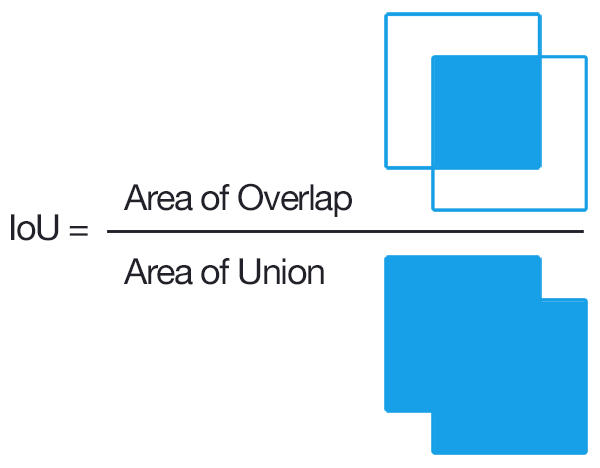
\includegraphics[width=0.3\linewidth]{img/Intersection_over_Union_-_visual_equation.png}
	\caption{Intersection over Union between regions. Source: Wikipedia, CC BY-SA 4.0}
	\label{fig:intersection_over_union}
\end{figure}



\chapter{Content-based image retrieval}

Image retrieval has been an active research field since the 1970s. The traditional approaches included manual annotation of the images by textual or numerical metadata. The user could then formulate a query against these annotations to retrieve relevant images. This approach is often referred to as Concept-based image retrieval.

There are several drawbacks to the textual or numerical annotations. First of all, wide human annotations are often needed to provide rich data for filtering. Annotations including also spatial information take more resources than only writing down present objects in the image. Also the images often include too many details (i.e. type, color, the shape of the objects), which may be impossible to comprehensive by human annotations.  The annotations may even change later: a different person may include different details/objects and may perceive their attributes differently. To search for an image, the user must know the exact terms the annotators used in order to be able to retrieve the images they want. As the last problem, we pose with human annotations is the scalability. As the amount of information increases every second, there is no human capability to hand process all the examples.

During the 1990s, content-based image retrieval (CBIR) emerged. In the CBIR approach, the images are indexed by features directly derived from their visual content using automatic or semi-automatic image processing techniques. Such indexing lacks building blocks as words as it on the other hand provides semantic information about the whole images or its regions. The attributes of images are complex functions of regions of the image or the whole image.

CBIR has received considerable research interest in the last decades. With the advancement in Deep Learning a new pool of possible complex functions to describe the images emerged. 

\subsection*{Task formulation}

% We consider a known set of images I and a query Q∈ I. We utilize a representation ^Q over Q, such that minimize search_rank(^Q, I). We define search_rank as an ordering function based on similarity function (or inverse of distance function). We focus on testing different representations ^Q for query Q.  


\chapter{Search by Object Location}

The first representation technique we aim to test is based on visual memory. The specific scene was previously seen (memorized) and we look for a match in the database. This approach corresponds to the usual abilities of visual memory - naming the objects and where they were positioned. Therefore, we focus on retrieving the matched scene based on the collage of the places of the objects in the canvas -- which correspond to the positions of the objects in the scene (see an example Figure \ref{fig:query_collage_comparison}).

\begin{figure}
\centering

\begin{subfigure}[t]{0.45\textwidth}
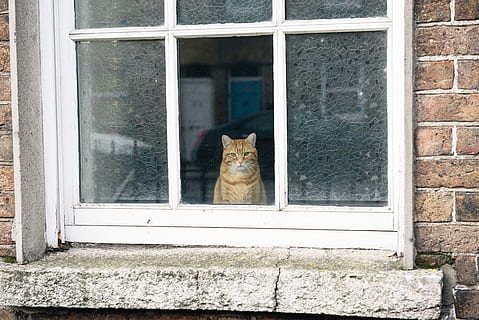
\includegraphics[width=0.9\linewidth]{img/cat_on_window} 
\caption{Query}
\label{fig:searched_scene}
\end{subfigure}
\begin{subfigure}[t]{0.45\textwidth}
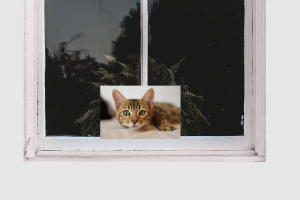
\includegraphics[width=0.9\linewidth]{img/cat_on_window_collage}
\caption{One of the possible collage description for the query}
\label{fig:collage_example}
\end{subfigure}

\caption{Example of searched scene (query) with possible visual description by a collage.}
\label{fig:query_collage_comparison}
\end{figure}


% First approach we explore is based on knowing the position of the objects in the image. This corresponds to a visual memory. People with a good visual memory are usually able to describe the position of the objects regarding to each other or in absolute way in the whole image. An example to this shows the image \todo[]{}.

% We aim to overcome a limitation on vocabulary size for common approach by description of words. We implement search only on visual requests, which, if takes rich enoucgh descriptors has significantly higher capability.

% % In the TrackVid competition, many presented solutions are limited and do not scale well. For example is keyword search, which is limited to the size of the vocabulary. In this chapter we overcome this limitation. We develop search based on images instead of words to avoid the vocabulary limit. We use state-of-art knowledge to acquire deep representation of the objects.

% % The second limitation we tackle is multi-query. It is difficult to find a source video if many scenes with the same type of the objects occur in the dataset (see Image ....). We solve this problem by placing multiple single queries and then using fusion to merge rankings from each query (more in ...).


% The research in the recent years showed, that neural networks purposfully trained for a set of objects can gain an ability to create a good representation also for unseen objects \todo[]{source}. In this thesis we work with this presumption and we work with these representations.

This approach aims to avoid the limitations of vocabulary size used to annotate the images. Even though recent advancements in the automatic capability of object detection as far as 1200 words \footnote{TODO} do not fully comprehend all diverse looks of the objects. For example, a single word for human may represent a visually wide range of possibilities, based on clothes, age, and other attributes. We aim to avoid this bottleneck and proceed with the search only on visual similarities to obtain a wide spectrum of possible queries.

In this chapter we utilise approaches based on two key information: 1. spatial information of the objects in the scene and 2. visual representation. Formally, representation $\hat{Q}$ of a query $Q$ is a set of pairs -- image and position. $\hat{Q} = \{ (pos_1, img_1), (pos_2, img_2), \dots \}$.

\section{User-program interaction}

The query is a collage of one or multiple images. Each image also includes its relative position in the canvas (i.e. how far it is from top left corner relative to the size of the canvas).

The user interacts with the environment by adding, scaling, and/or moving images. Interactively, the closest representatives found in the dataset are returned. The user can select the final image, if they think they found the corresponding scene. 

The figure \ref{fig:query_collage_comparison} shows an example of the query. The goal is to be able to use any of the currently available image search engines to create a collage. The user places multiple images onto the canvas. Their position on the canvas is recorded and later used to target the database in regard to their position. 

\section{Splitting an Image into Regions}

% In our first approach we cut the image into fixed regions. We aim to capture the 
% representation of each of these regions. This offers us an information specific for each region.

% With the query we can compare the features representation of the query and of the particular regions we are interested in.

% Image
% - Split to nxm regions
% - Compute deep representation for each of the regions

% Query
% compute deep representation for the image in the query
% for each image in the database, compare this representation to the representation of the region with highest IoU

% In our first approach we split the image to a regions. We compute a deep representation using neural network for each region and the whole image. 

One of the natural ways to capture spatial information about the objects in the scene is to cut the images into fixed regions. We then can capture visual information for these regions separately. For the incoming queries, we may compare the visual information of the query only to the regions which collide in the zone of the interest.

We split each image  $img \in D$ in the database into $N \times M$ regions. To provide full information about the image, we make an requirement for the regions to cover the whole image. To preserve square shape of the regions and also an option to obtain more information, we allow overlaps between the regions. For each of the newly region $r_{img, i, j}$ we preserve information about its original image $img$, region’s position (coordinates of the region $i, j$) and visual features $f(r_{img, i,j}$.



% \section{ Using Deep Representation}
%   - Using Deep Representation
%       = Using antepenultimate layer of classification networks

% \section{Multi-query search}
% - Multi query search
%   - Fusion methods
%   - Comparison of both approaches with multimodal performance over different fusion techniques

% Our work focuses on difficult to describe scenes with multiple easy to recognize objects. In this questions a natural question of how to rank the results based on multi query.

% In this section we go through several approaches we tested. We base our 

% \subsection{Fusion Methods}

% \section{Evaluation}
% In this chapter we evaluate all previously mentioned approached. Firstly, we describe our methodology behind the experiments and then we proceed through all approaches. 

\subsection{Regions Shape}

In order to use transfer learning for common CNN and to avoid additional skewing in resizing, we limit to the regions only to the shape of squares. Since this input size of the square is one of the parameters, we aim to use the size of the squares the same as the size of the input of the network. This helps us to avoid unnecessary scaling which may be introduced when the length of the side of the square does not match with the input for the network.

With fixed-width $w$ of the square and the number of regions $N \times M$, we define the following regions:
\[ 
r_{i,j} = {(( \text{image\_height} - w) / (n - 1) *i, ( \text{image\_width} - w) / (m - 1) * j)}
\]

With the condition on full coverage of the image (i.e. \(w n >= \text{image\_height}\), and for $m$ respectively) we obtain full coverage of the image by the regions. Overlaps are evenly distributed over both axis.

\begin{figure}
\centering
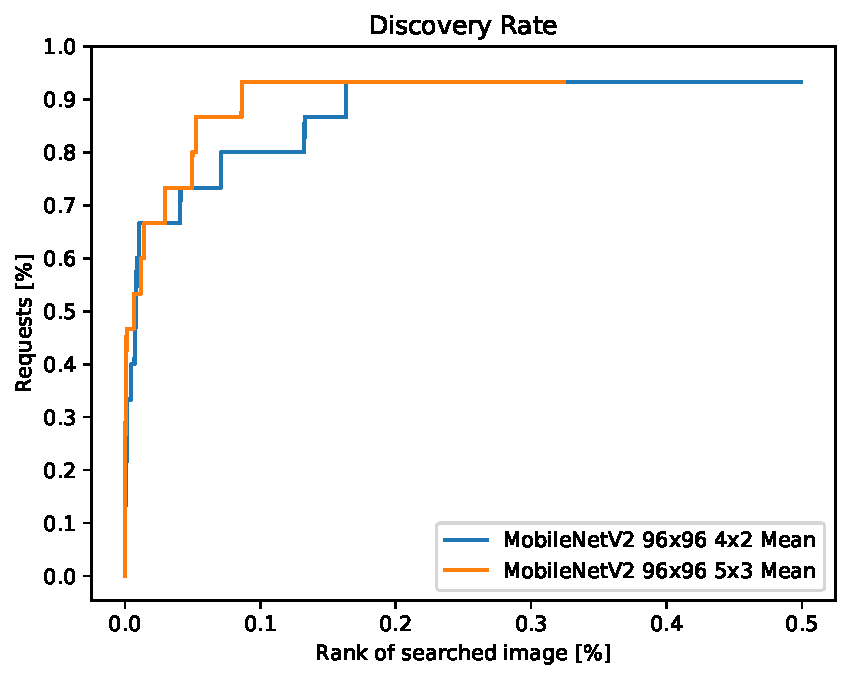
\includegraphics[width=\textwidth]{graphs/78f2a977489ac08dddac6f53446b388292306ec95f9dcbc7ca8359fbedfed9b0}
\caption{Performance of the system based on different number of regions per image}
\label{fig:different_number_regions}
\end{figure}

\subsection{Choice of regions}

Given one incoming query image with its position and shape we propose several methods for choice of the “targeted” regions. For each one of the fixed regions we compute %\[\text{IoU_{i,j,k}} = \text{IoU}(Ri,j; Qk) for all i, j. \]

First of the options, is to only compare the region with highest Intersection over Union, limiting to the argmax IoUijk. I.e. for each i belongs I only one region would taken into account.

Second approach is to collect all intercepted regions for the similarity. This is an exhaustive process. This may result in increased computation time, i.e. usually from 2 to 9 times slower. In case of a huge set of data without any indexing, it may increase time of a request from 1 sec up to several seconds.

Third choice is to limit the number of targeted regions to a certain number. This offers us an advantage of fuller coverage and possibility for better match in neighbouring region, on the other hand provides an upper bound for the computational time required per request. 

Visualisation of chosing different number of crops can be seen in figure \ref{fig:fish_with_grid}. A comparison of the performance dependend on different number of chosen crops is shown in figure \ref{fig:crop_limitation}.

\begin{figure}
\centering
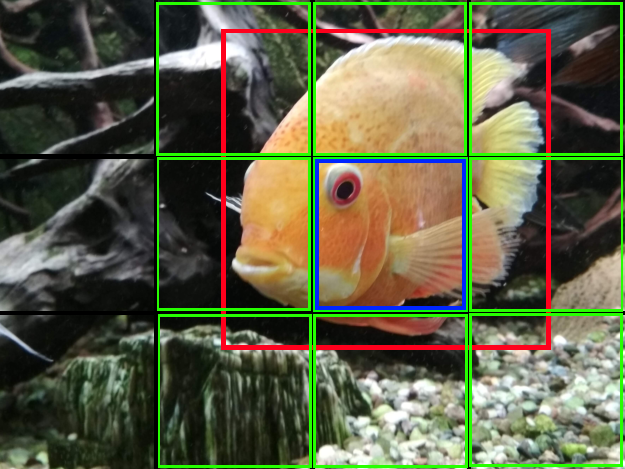
\includegraphics[width=0.6\textwidth]{img/fish_grid_regions}
\caption{Example of choosing the corresponding regions. Red: query position; Green: all intercepted regions; Blue: region with highest IoU.}
\label{fig:fish_with_grid}
\end{figure}


\begin{figure}
\centering
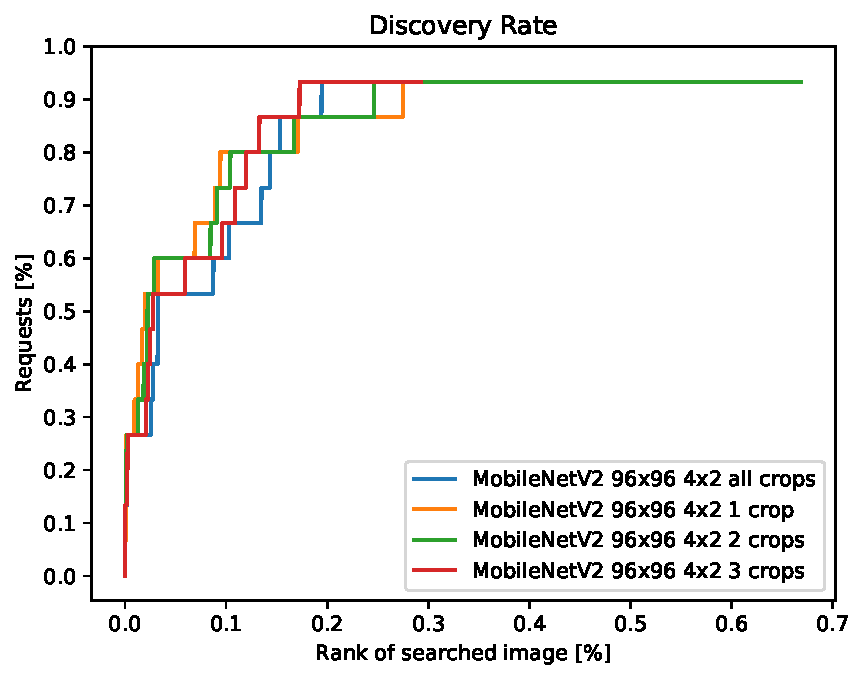
\includegraphics[width=\textwidth]{graphs/c2cf4e147040018e6cfc46043bb59de4f5f3e83441c1e1024af0b7bab644a994}
\caption{Performance of the system based on different number of chosen crops}
\label{fig:crop_limitation}
\end{figure}


\section{Using more information from antepenultimate layers from CNN}

The previously mentioned approach has a shortcoming. It is not able to grasp the arbitrary position of the object, rather it has limitations to previously fixed regions. This may lead to decreased performance for the objects, which cover a bigger part of the scene, i.e. in the previous case, it may overlap over multiple regions. This brings not only computational disadvantages but also reduces the amount of information which are used when compared to the query.

We propose an approach, where an antepenultimate layer of common CNN's may be used. Common CNNs are built out of several building blocks, i.e. convolution layers intervened by pooling (TODO image). This approach proved its ability for image recognition and many other related tasks (TODO add source). Many of the current state-of-the-art models use the pooling layer before fully connected layer for categorization.

We aim to leverage this antepenultimate layer, which contains not only visual features but also spatial information.

\subsection{Choosing region of interest in the layer}

Layers before pooling on which we focus are 3 dimensional. First two dimensions contain spatial information, which is propagated from the previous layers. The third dimension contains visual information.

In order to obtain only a part of this layer we are interested in (i.e. our query was placed in that specific region) we need to take only a subset over first two dimensions. For a query defined by Qi = (y, x, h, w) and layer Li with first two dimensions H, W we consider a Li[y * H, x*W, (y+h) * H, (x + w) * W]. 

It is important to notice, that these layers use to have significantly lower height and width, compared to the input of the network. For example, before-last-pooling layer of Resnet50V2 has dimensions (7,7,2048). Therefore, we round our subset to nearest whole number and in case of no intersection we maintain at least intersection of size 1x1.

After this choice of the region of interest, we continue with the pooling layer in order to obtain one feature vector.

In comparison with the previous Splitting in regions approach, we see an enhanced ability to grasp more variability in object position. Especially, in queries which overlap most of the regions. On the contrary, this approach may require more memory, as for comparison for Resnet50V2 with 12 regions we needed to work only with 12 feature vectors. With the before-last-pooling layer we need for Resnet50V2 to work with 49 feature vectors. This may not be limitation with smaller feature vectors, but may come as a practical limitation based on the size of the dataset and computability power available.


\section{Ranking}
In the previous sections, we talked about the obtaining feature vector for the items in the database of the regions we are interested in. In this section, we take a closer look on further processing these obtained feature vectors.

Assuming we have an image for the query, we use the same model to compute the feature vector as was used to precompute the features for the database. Based on that we define a distance D, as the distance between the feature vector of the query and feature vector of the item in the database. This comparison to each database item gives us the distance between each item in the database and our query image.

Based on these distances we order the results, starting from the lowest to the highest distance. This distance acts as an inverse for the similarity. Similar to the results are, lower is the distance.

We use 3 main distance metrics:
Cosine Distance
Euclidean L2 distance
Euclidean L1 distance

\section{Multiple objects in the scene}

So far we talked only about handling queries consisting of one searched object. This limitation is very strict and therefore we experiment with multiple approaches to index the database based on multiple objects in the scene.

Firstly we make an assumption, that all query images have the same importance and are expected to be with the same level of relevance. Therefore we approach this problem as a set of query images, rather than as an ordered list.

We work further only with already precomputed rankings with corresponding distances for each image/part of the image. We propose several ways to merge the rankings.

We define ranking $R$ as a set of distances between the query image $q$ and database item $i$. We look for a function \(r: R^n -> R\), which merges multiple rankings into one final ranking. Our goal is to minimize rank for each of the queries in the test items.

We tested several functions for this role and to compare a function that does not take into account the distances with different functions over the distances. A comparison for MobileNetV2 can be seen in figure \ref{fig:ranking_funcs}.

\begin{figure}
\centering
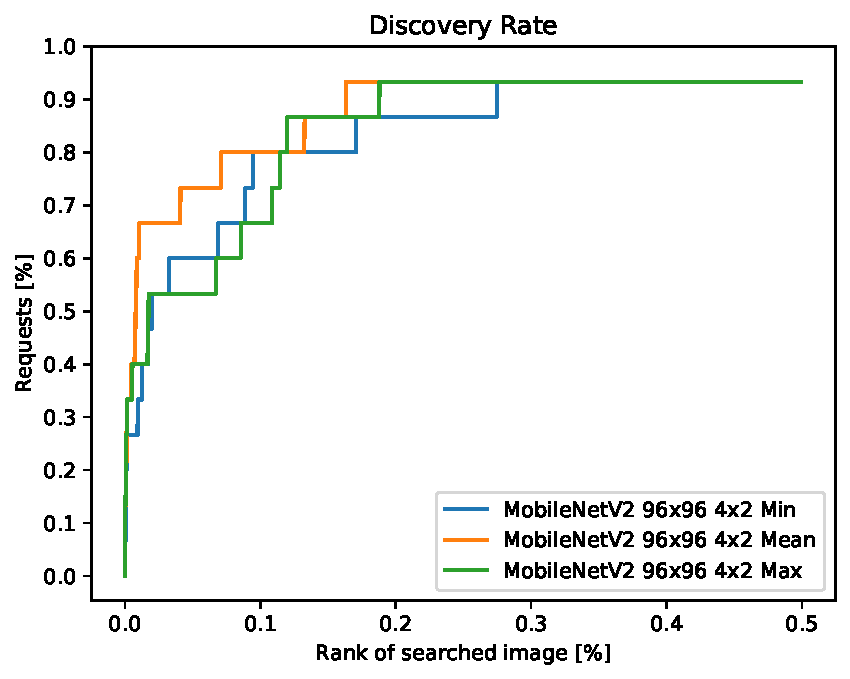
\includegraphics[width=\textwidth]{graphs/362cb9a687ce05c7732f973defca88fb8c5c393f5992066521343314698c9de7}
\caption{Performance of the system based on different fusion method}
\label{fig:ranking_funcs}
\end{figure}





